\chapter{\label{II_3}Indexation des données produites au sein du modèle de données} 
\titreEntete{Indexation des données produites}

L’objet de notre étude est le reversement des données produites par l’indexation automatique au sein du modèle FRBR, adapté aux archives audiovisuelles. Si les outils d’extraction automatique tels que YOLOv8, nécessitent un réentrainement spécifique au corpus étudié, une seconde difficulté s'impose, celle de l'alignement de ces données avec un modèle de données personnalisé. Le modèle de données FRBR est, en effet, configuré selon les besoins métier de chaque institution et conditionne l’organisation des données pour l’utilisateur au sein de l’interface. Dès lors, comment reverser des données produites automatiquement, au sein d’un modèle de données configurable ? Ce reversement concrétise en effet l’indexation automatique, puisque les données deviennent visibles et requêtables par les utilisateurs, au sein de l'interface du logiciel. 

%Faire le lien avec le NLP le plus possible : le NLP pourra être étendu pour la recherche de contenus visuels  

%Yolo est une IA discriminative 


\section{\label{II_3_A}Reversement des données au sein du FRBR} 

Le processus automatisé proposé repose sur l'exécution de deux phases : d'une part la segmentation temporelle d'un flux vidéo (géérant des time codes et des images-clé), et d'autre part la détection et la classification d'objets (générant des mots-clés). L'enjeu est de prévoir la structuration de ces différents types de données, chiffrées et textuelles, au sein du modèle FRBR existant. 

%Certains outils ont déjà été développés dans d’autres applications de gestion des collections afin d’effectuer ce reversement de manière automatique : Wedia, Keepeek, Einden, MomaSoft “classent automatiquement les images et vidéos en leur attribuant les métadonnées appropriées.” \footcite{zotero-item-732}

Les outils automatiques utilisés lors du processus ont extrait des données depuis un média, associé au niveau de l'item numérique au sein du modèle de données préexistant. Or, le niveau item contient des éléments de description matérielle techniques, alors que les mots-clés et repères temporels relèvent d'une description intelectuelle et syntaxique. Dès lors, la création d'une entité intelectuelle dédiée à la séquence s'impose. 
Afin d'illustrer l'intégration d'une entité de description intermédiaire, entre l'oeuvre et l'item numérique, prenons l'exemple de la plateforme Okapi (Open and Knowledge-based Annotation and Publishing Interface), développée par le département Recherche et Innovation de l'\gls{ina} \footcite{lalande2022}. Afin de favoriser la description collaborative de contenus multimédias, la plateforme offre la possibilité aux utilisateurs de concevoir des modèles de description personnalisés \footcite{lalande2022}. La plateforme permet notamment de séparer l'extrait audiovisuel du média, dont il constitue un niveau descriptif propre. Une strate supplémentaire de description est ainsi dédiée à la description intellectuelle du média. Le modèle FRBR tel que nous l'avons décrit ne propose, a priori, pas d'entité descriptive dédiée à la séquence. L'entité "d'agrégats", proposée par le manuel de la \gls{fiaf} pourrait y correspondre. Toutefois, ceux-ci “sont conçus et créés dès le début pour rassembler plusieurs composantes individuelles formant un tout." \footcite{zotero-item-646}. Or, au sein du corpus étudié, les rushes ne font pas partie d'un montage. Toute segmentation est une interprétation a posteriori de la construction de l’archive, et donc un remontage. L'entité de "fragment d'expression" proposé par l'IFLA au sein du modèle FRBR bibliographique semble plus adéquate \footcite{iflastandards.info2026}. L’\gls{IFLA} définit le fragment comme “des parties d’expressions qui ne constituent pas elles-mêmes des expressions autonomes.[...] Un « Fragment d’expression » n’est identifié qu’en fonction de son occurrence au sein d’un tout connu ou supposé.” \footcite{iflastandards.info2026}. Cette entité semble correspondre à la notion de séquences telle que nous l'avons décrite. Elle serait rattachée à l’Oeuvre, conformément à l’adaptation du FRBR par les recommandations de la FIAF, et permettrait le reversement spécifique des times-codes et mots-clés. La figure \ref{figfragment} ci-dessous illustre l'intégration de l'entité du fragment d'oeuvre au modèle de données existant. 

\begin{figure}[htbp] 
	
	\centering 
	
	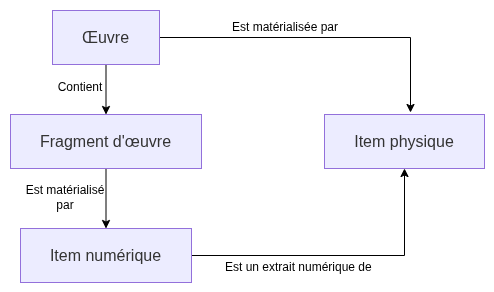
\includegraphics[width=0.7\textwidth]{images/fragment_frbr.png} 
	
	\caption{Intégration du Fragment au modèle de données} 
	
	\label{figfragment} 
	
\end{figure} 

Au sein de la plateforme Okapi, la création d'une entité intermédiaire de description, permet aux données descriptives produites à partir du média, d'être reversées au sein d'un niveau parent essentiellement descriptif, celui de l'extrait. Au sein du modèle de données existant, adapté au corpus étudié, les time codes et les mots-clés sont déjà indexés manuellement en tant que données au sein de l’application. En effet, les times codes sont renseignés au niveau de l'item numérique, dans un champ notes, et l'item comporte le champ type renseigné par la valeur “fichier time codé”, afin de signifier sa qualité d'extrait. De plus, les mots-clés sont renseignés au niveau de l’indexation de l’œuvre, donc du rush original. La modélisation de la segmentation au sein du modèle actuel implique un nombre conséquent de relations entre les éléments, complexifiant ainsi la navigation de l'utilisateur. En effet, une notice d'item physique renseigne tous les extraits numériques (items numériques) qui lui sont liés. L’item numérique (segment) renseigne le film physique duquel il est extrait, tandis que le niveau œuvre renseigne uniquement les extraits numériques qui lui sont associés. 
La création d’une nouvelle entité simplifierait la navigation au sein de l'interface et permettrait de séparer la description en différents niveaux, intellectuel et technique, conformément aux principes du FRBR. La nouvelle entité de fragments permettrait éventuellement de préciser un contexte de segmentation et des champs dédiés aux mots clés et aux time codes. Le tableau \ref{tab:reversement_metadonnees_frbr} ci-dessous illustre la répartition de la description entre le fragment d'Oeuvre et l'item numérique. Pour des raisons de clarté, d'autres données descriptives ont été intégrées afin d'illustrer la répartition entre la description intellectuelle et matérielle. 

\begin{table}[H]
	\centering
	\small
	\renewcommand{\arraystretch}{1.3}
	\begin{tabular}{|p{3.8cm}|p{4.2cm}|p{6.4cm}|}
		\hline
		\textbf{Entité FRBR} & \textbf{Champ / Attribut} & \textbf{Exemples de valeurs} \\
		\hline
		\multirow{6}{=}{\textbf{Fragment d’Oeuvre} \newline \textit{(Description intellectuelle)}} 
		& Contexte & Segmentation automatique de tel item physique \\ \cline{2-3}
		& Description générale & Description du contenu sémantique de la séquence \\ \cline{2-3}
		& Processus de segmentation & Automatique (Outil utilisé et paramètres appliqués) \\ \cline{2-3}
		& Time codes & Time codes de début et de fin de la séquence \\ \cline{2-3}
		& Mots-clés & Mots-clés extraits par YOLO \\ \cline{2-3}
		& Image-clé associée & Lien direct vers le fichier de l'image-clé \\ \cline{2-3}
		& Oeuvre parente & Identifiant de l'oeuvre associée, lien direct vers la notice \\ \cline{2-3}
		& Item physique associé & Identifiant de l'item physique associé dont est tirée la séquence, lien direct vers la notice \\ \cline{2-3}
		& Item numérique associé & Identifiant de l'item numérique associé, lien direct vers la notice \\ 
		\hline
		\multirow{3}{=}{\textbf{Item Numérique} \newline \textit{(Description technique et matérielle)}} 
		& Fragment associé & Identifiant du fragment associé, lien direct vers la notice \\ \cline{2-3}
		& Données techniques & Résolution de l'image, taille, format \\ \cline{2-3}
		& Données de conservation & Emplacement, contenant \\ \cline{2-3}
		& Média associé & fichier média de la séquence \\ \cline{2-3}
		\hline
	\end{tabular}
	\caption{Attributs et exemples de valeurs associées aux entités Fragment d'Expression et Item Numérique.}
	\label{tab:reversement_metadonnees_frbr}
\end{table}

Les métadonnées automatiquement produites seraient intégrées au niveau du fragment, tandis que l'item numérique contiendrait le média et les données techniques. 
Une difficulté subsiste toutefois. En effet, les processus s'exécutent au niveau du fichier numérique et de son média, tandis que les métadonnées produites doivent pouvoir enrichir un niveau descriptif supérieur, celui du fragment. Dexu configurations peuvent être envisagées afin d'opérer ce reversement automatiquement. D'une part, l'application gère actuellement l'héritage des données d'un niveau supérieur à un niveau inférieur via la configuration de méta-masques, qui ciblent les niveaux iférieurs au sein desquels reverser les données. Néanmoins, le processus automatisé décrit impliquerait la configuration de masques ascendants, permettant de reverser des métadonnées générées au niveau de l'item, vers l'entité de fragment. Cette configuration complexifie toutefois la compréhension du modèle de données.
D'autre part, pourrait être envisagé la mise en place d'un tableau de correspondance ou d'un script permettant d'associer les sorties de données du processus aux entités dans lesquelles elles doivent être injectées. 
Une fois la modélisation du transfert établie entre les métadonnées automatiquement produites, et le modèle de données existant, le reversement définitif est toutefois laissé à l'utilisateur métier, au sein de l'interface du logiciel. 
%À l’ingest : données interdépendantes entre la description d’un item numérique et de son média. Mentionner la relation nouvelle sur l’item numérique et son média : facilite les choses pour le reversement  
%Pour les times codes, des champs dédiés devrons être prévus sous le champ film associé.  
%Faire un schéma de métadonnées pour pouvoir adapter les données aux normes du logiciel via des connecteurs par exemple.  

\section{\label{II_3_B}Proposer une interface de validation pour l'utilisateur} 

Si la redéfinition du modèle \gls{FRBR} s'effectue en \textit{backend} de l’application, par les équipes techniques et les équipes métiers du logiciel, afin de préparer l’implémentation de processus automatiques, les étapes de ces processus doivent toutefois être restituées au sein de l'interface auprès de l'utilisateur métier. Afin de donner à l'utilisateur le rôle de validation finale sur les données produites, l'espace de travail S-Movies doit permettre de visualiser les résultats afin de les valider. 

\subsection{Un enjeu de transparence}

En effet, dans le cadre de l'implémentation de fonctionnalités automatiques, fondées sur l'intelligence artificielle, la \gls{cnil} recommande que les utilisateurs soient familiarisés au fonctionnement et aux limites de ces outils, par exemple “la manière dont sont produites les sorties, les éventuels transferts de données, ainsi que les usages autorisés et les usages interdits." \footcite{zotero-item-729}. Ces informations pourraient notamment guider l’utilisateur pour la validation des données produites par les modèles. Si l'exposition de ces étapes peut être effectuée au sein de modes d'emploi dédiés, comme Skinsoft le prévoit déjà, les informations relatives aux fonctionnalités automatiques devront toutefois être directement intégrées à l’interface pour un souci de transparence. Ainsi, la \gls{cnil} recommande que "l’intégration de briques d’IA générative dans un système d’information (SI) devrait être pensée avec des éléments de design informant clairement les utilisateurs de l’origine de la proposition [...]." \footcite{zotero-item-729}.
De plus, en cas de non-validation des données produites par l'utilisateur, il pourrait être pertinent de proposer "un point de contact pour remonter des problèmes ou des difficultés d’ordre éthique"\footcite{zotero-item-729}. L’interface devra ainsi prévoir un formulaire décrivant la raison du refus des données, envoyé à l’équipe technique afin que l'algorithme puisse être amélioré, voire affiné. Au cours de notre stage, un système similaire a été proposé afin de prévoir la gestion des erreurs d'un outil de recherche en langage naturel, visible en Annexe B (\ref{annexe_B}). Un formulaire est prévu pour l'utilisateur en cas de résultats non pertinents pour que le processus soit amélioré.

\subsection{Développer une interface dédiée à la validation de l'utilisateur}
Si notre étude ne relève pas de l'\gls{ia} générative, il est toutefois pertinent d'offrir à l'utilisateur un niveau de transparence maximal au sein de l'interface, via la viualisation des données produites et leur validation finale. À l'image des deux phases de traitement automatiques développées dans les sections précédentes (segmentation et classification), la validation côté interface pourra prendre la forme de deux phases de décision. Il pourra d'abord être demandé à l'utilisateur d'actionner ou non le processus de segmentation puis de le valider ou de l'invalider. Une fois le processus de segmentation finalisé, l'utilisateur pourra décider de déclencher le processus de détection d'objets sur les segments produits, puis de finalement les modifier ou de les valider.
Afin de concrétiser le processus de validation côté interface, nous nous appuyons sur l'exemple de la plateforme Amalia.js, développée par l'\gls{ina} en 2015, conçue pour visualiser les résultats d’algorithmes d’analyse audiovisuelle \footcite{zotero-item-740}. Le besoin à l'origine d'Amalia.js est donc de permettre de visualiser les résultats divers issus de pipelines d'automatisation \footcite{herve2015}. Cette interface permettrait d'une part de visualiser les résultats et d'autre part, de vérifier la conformité des données produites en lien avec les standards métiers en vigueur au sein du logiciel \footcite{herve2015}. L'interface permet également d’annoter directement le flux vidéo afin de corriger les données produites \footcite{herve2015}. La correction effectuée par l'utilisateur  permet de constituer des données d'entraînement supplémentaires afin d'améliorer les algorithmes d'indexation automatique \footcite{herve2015}. 
Amalia.js intègre notamment un \textit{plugin} de \textit{timeline} pour l'affichage des segments temporels et des images-clés associées, ainsi qu'un \textit{plugin} de superposition (\textit{overlay}) qui permettrait l'affichage de l'encadrement des objets détectés \footcite{zotero-item-740}.
Plutôt que de développer deux modules distincts, cette logique pourrait être combinée au sein de S-Movies sous la forme d'un module d'édition des données. Ce module présenterait d'abord à l'utilisateur la ligne temporelle des séquences associées aux images-clés, puis après leur validation, le module prévoierait l'ouverture d'une fenêtre d'édition latérale contenant les propositions de mots-clés et les objets détectés entourés au sein des images-clés. Ce module d'édition s'inspire du \textit{plugin} \textit{Editor} au sein d'Amalia.js dont la figure \ref{figamalia} ci-dessous ilustre la disposition : 

\begin{figure}[H] 
	
	\centering 
	
	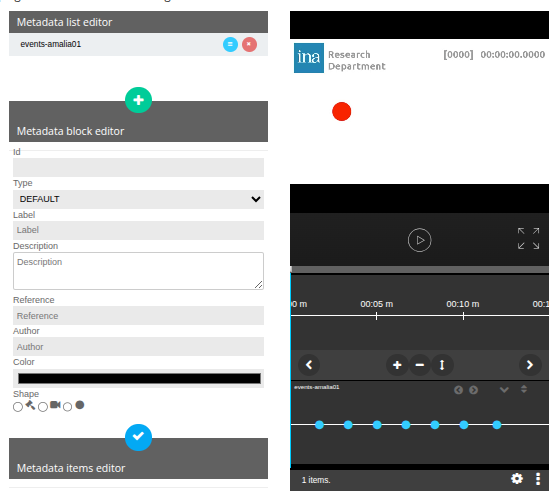
\includegraphics[width=1.0\textwidth]{images/amalia.png} 
	
	\caption{\textit{Plugin Editor} dans Amalia.js \footcite{zotero-item-794}} 
	
	\label{figamalia} 
	
\end{figure}

En cas de modification par l'utilisateur, l'interface pourrait enregistrer les données validées, tout en les envoyant en \textit{backend}, afin que le processus soit amélioré. 
Le développement de l'interface serait ainsi conforme à la mise en place d'une automatisation facilitatrice de la création de données, en incitant l'utilisateur "à vérifier les données fournies en entrée et la qualité des sorties" \footcite{zotero-item-729}.

\subsection{Déroulé du processus de validation}

Concrètement, en \textit{frontend}, dans l’interface de l’application prévue pour l’utilisateur, le processus suivant peut-être imaginé, illustré par un diagramme de décision (\ref{fig:validation}):

\begin{figure}[H] 
	
	\centering 
	
	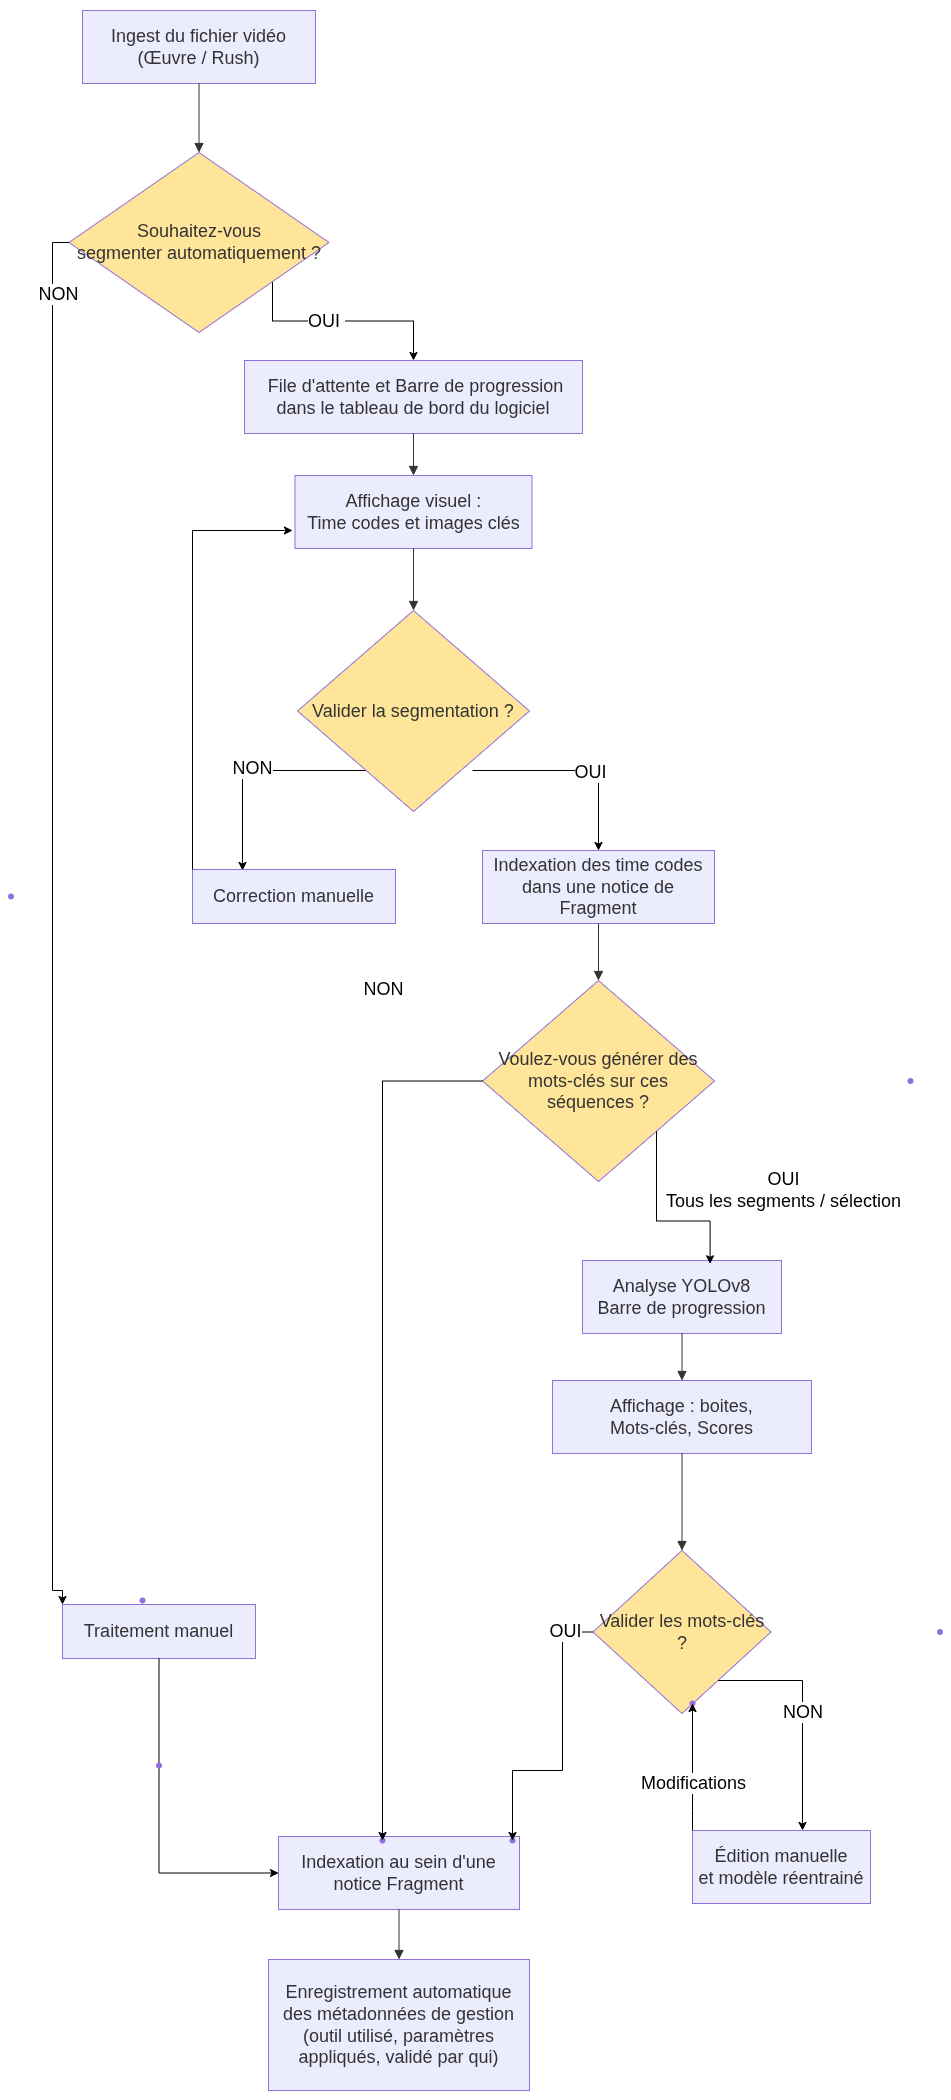
\includegraphics[width=0.6\textwidth]{images/validation.png} 
	
	\caption{Processus de validation de l'utilisateur métier} 
	
	\label{fig:validation} 
	
\end{figure}

Ce processus permet de laisser l'utilisateur métier décider de l'indexation des données via l'actionnage ou non des fonctionnalités automatiques. L'utilisateur décide en amont du processus, et valide ensuite les données produites à es fins d'indexation. 

%Exemple de la plateforme okapi :  

%“Okapi fournit un ensemble d’outils destiné à l’analyse sémantique et sémiotique de contenus multimédia (vidéo, image, son) et à la gestion de corpus de vidéos, d’extraits sonores et de parties d’images. Les outils d’analyse permettent l’indexation et la description sémantique de contenu sur la base d’ontologies qui décrivent les objets et classes des domaines étudiés. Les outils de gestion de corpus fournissent des services pour la constitution, la visualisation, l’enrichissement et la valorisation de corpus thématiques.” \footcite{lalande2022} (cf capture d'écran)
\section{\label{II_3_C}Rendre les données recherchables et découvrables} 

Une fois les données validées et indexées au sein du modèle de données, elles modifient l'accès aux archives. L'indexation de séquences décrites par une nouvelle entité de description, permet à  l'institution de non plus seulement avoir accès aux archives dans leur globalité, mais à une "indexation fine" de leur contenu \footcite{bachimont2007}. Ainsi, par une recherche de mots-clés, l'utilisateur peut directement accéder aux segments d’archives concernés. La modélisation descriptive prévue par le FRBR permet de conserver le contexte du fragment, associé d'une part à l'oeuvre dont il est extrait, et d'autre part au média numérique associé. Les liens entre le fragment et les entités liées sont toujours requis, empêchant ainsi un risque de désolidarisation du contexte. 
Les séquences créées par le processus automatique pourront ainsi être requêtées par l'utilisateur via les outils de recherche offerts par le logiciel développé par Skinsoft. En effet, le logiciel propose les modes de recherche suivants : recherche simple, recherche avancée, recherche plein texte ciblée, recherche par image. De plus, une recherche en langage naturel, basée sur le \gls{nlp} et sur une génération augmentée de récupération (\gls{rag}), imaginée au cours de notre stage, est en cours de développement au sein du logiciel.  
Ce mode de recherche permet à l'utilisateur de formuler des requêtes complexes en langage naturel, afin d'améliorer l'expérience de navigation au sein de l'interface. L'utilisateur, via ce mode de recherche, n'a plus besoin d'employer les mots-clés exacts pour obtenir certains résultats. Par exemple, il peut formuler la requête suivante : "toutes les archives sur des défilés militaires". Le moteur effectue ensuite le lien entre la formulation de l'utilisateur en langage naturel, et les mots-clés indexés sur les séquences. Les résultats de recherche pourront par exemple présenter les séquences contenant les mots-clés suivants : "foule", "drapeau", "armée", "police". Une fois les résultats de recherche présentés, l'utilisateur peut cliquer sur une notice et accéder directement au média lié à une séquence spécifique, au sein d'une grille de recherche. Cela permet une large découvrabilité des archives, concrétisant ainsi les besoins utilisateurs fondateurs du modèle FRBR, de "trouver, identifier, sélectionner, obtenir" \footcite{zotero-item-653}. 
Les résultats de recherche pourront présenter en vignette, l’image clé associée au segment décrit, sur laquelle l’utilisateur peut cliquer. 
Outre la recherche textuelle, l'indexation fine des contenus audiovisuels peut développer l'usage d'autres modes de recherche visuels innovants. Le moteur Snoop, développé conjointement par l'\gls{ina} et l'Institut national de recherche en informatique et en
automatique (\gls{inria}), permet de croiser une exploration fine des contenus audiovisuels avec une interactivité qui place l'utilisateur au centre \footcite{zotero-item-744}. Fondé sur un bouclage de pertinence, il permet, à partir d'une requête sur une caractéristique visuelle, de proposer à l'utilisateur des résultats pertinents que celui-ci peut annoter comme résultats pertinents ou non pertinents \footcite{zotero-item-796}. Le moteur prend ces annotations en compte afin d'affiner la pertinence des résultats de recherche.
Ce moteur innovant suit la même logique que l'interface de validation pensée sur le modèle d'Amalia.js, et que le mode de recherche en \gls{nlp}, qui prévoit d'être affiné en fonction des retours utilisateurs. Les retours utilisateur, intégrés à l'interface, ne srevent pas seulement à valider les données mais améliorent le fonctionnement du logiciel, fond sur des processus automatisés. 

Conclusion sous partie 
\textit{In fine}, l'intégration de l'indexation automtique au sein d'un logiciel de gestion des collections exige une réadaptation du modèle de données via la création d'une nouvelle entité qui permet d'accueillir adéquatement les nouvelles métadonnées produites. De plus, l'implémentation du processus automatique implique la mise en place d'une interface de validation qui place l'utilisateur au centre de l'indexation définitive. Une fois indexées, la masse de données produites permet de concrétiser la finalité du FRBR, celle de la découvrabilité, via des outils de recherche innovants qui permettent d'explorer directement le contenu de l'image. 


\textit{In fine}, l'intégration de l'indexation automtique au sein d'un logiciel de gestion des collections exige une réadaptation du modèle de données via la création d'une nouvelle entité qui permet d'accueillir adéquatement les nouvelles métadonnées produites. De plus, l'implémentation du processus automatique implique la mise en place d'une interface de validation qui place l'utilisateur au centre de l'indexation définitive. Une fois indexées, la masse de données produites permet de concrétiser la finalité du \gls{FRBR}, celle de la découvrabilité, via des outils de recherche innovants qui permettent d'explorer directement le contenu de l'image. 



%"Si l’utilisation envisagée consiste à fournir des données personnelles (données des clients ou des collaborateurs) ou de la documentation sensible ou stratégique (par exemple pour le RAG), il semble généralement plus opportun et plus sécurisé de privilégier le déploiement de solutions « sur site » (on premise) qui présentent l’avantage de limiter les risques d’extraction de données auprès d’un tiers" \footcite{zotero-item-729}
%"s’il est envisagé d’utiliser un système sous forme d’API, il faut souligner que la maîtrise du système est alors quasi exclusivement dans les mains du fournisseur. Il convient donc d’être particulièrement vigilant sur les données soumises au système d’IA" \footcite{zotero-item-729}

%Le besoin à l'origine d'Amalia.js est de permettre de visualiser les résultats de pipelines d'automatisation, avec leur lot de métadonnées produites : « Whatever the field of analysis, we always need to be able to quickly and easily view the results of the methods we are developing. This problem is particularly true as we often manipulate large amount of videos. Developing visualization and annotation tools is often a tedious task that deserves to be pooled. »\footcite{herve2015}
%« The analysis being at different levels (keyframes, video segments, audio channels, associated synopses, one video alone or relative to a corpus...) results are obtained in very different natures, often needing quite specific approaches to be presented to the end user. »\footcite{herve2015} L'indexation utomatique regroupe tout un tas de métadonnées issues d'algorithmes et d'outils différents qu'il faut réunir dans ne interface de présentation. 

%"A major challenge for making AVP tools available
%is that the underlying algorithms need direct access to the data, yet due to strict IPR regulation this data often cannot leave the archives’ digital environment. A side effect of this is that for the analysis of AV material commercially available tools cannot be used, as these are primarily cloud based. it is necessary that any AVP infrastructure can be integrated with a local archival infrastructure, i.e., we need to bring the algorithms to the data, rather than the data to the algorithms." \footcite{noord2021}. Solution : projet CLARIAH 

%"Moreover, DANE is designed
%to be able to function in environments where there are fewer compute resources, or environments where access to the data is rate limited, as is typical for AV archives. To make this possible, the DANE architecture (as shown in Figure 2) divides the tasks to be performed over different workers that perform one specific type of analysis, where the work is assigned to a worker by means of message broker queuing system. The results of the analyses are communicated back to the server by the workers, and made available via an API to clients (e.g., other services or individual users)." \footcite{noord2021} (+ schéma qui montre l'architecture)

%"To enrich the AV collections in the Media Suite with automatically generated (and time-coded) metadata an assortment of AVP tools had been added to DANE, ranging from Semantic Object Detection, to colour analysis, to Automatic Speech Recognition."\footcite{noord2021}

%"These tools generate two types of metadata: (i) structured data which can be integrated into the existing metadata systems, and (ii) feature vectors which describe the data on a more abstract level, but which can be integrated in new types of interfaces and search systems. For instance, with an Object Recognition model it is possible to recognise which objects are present in an image, but the output of such a model can also be used to perform more abstract visual similarity queries" \footcite{noord2021}

%exemple d'indexation automatique à la bibliothèque nationale de finlande "L’API « suggest » est au cœur de ce web service : en fournissant un document textuel en entrée, on obtient en sortie une liste (au format JSON) de suggestions de concepts pour l’indexer ainsi que l’appréciation quantifiée de leur niveau de pertinence. Autre fonctionnalité importante, « learn » est capable de mettre à jour les programmes en exploitant des correspondances vérifiées entre des documents décrits et les mots sujets choisis."\footcite{suominen2019a}ss